\documentclass{vldb}
\usepackage{graphicx, subfigure, multirow, times}
\usepackage{balance, url, amsfonts, verbatim, mathtools, draftwatermarktop, draftwatermarkbottom}  % for  \balance command ON LAST PAGE  (only there!)

    \renewcommand{\topfraction}{1}	% max fraction of floats at top
    \renewcommand{\bottomfraction}{1}	% max fraction of floats at bottom
    %   Parameters for TEXT pages (not float pages):
    \renewcommand{\dbltopfraction}{1}	% fit big float above 2-col. text
    \renewcommand{\textfraction}{0.5}	% allow minimal text w. figs
    %   Parameters for FLOAT pages (not text pages):
    \renewcommand{\floatpagefraction}{0.7}	% require fuller float pages
	% N.B.: floatpagefraction MUST be less than topfraction !!
    \renewcommand{\dblfloatpagefraction}{0.7}	% require fuller float pages

  \renewcommand{\ttdefault}{cmtt}


\usepackage{mdwlist}

\title{Probabilistically Bounded Staleness and\\ Practical Partial Quorum Systems}

\author{Peter Bailis, Shivaram Venkataraman, Michael J. Franklin, Ion Stoica, Joseph M. Hellerstein\\
\affaddr{University of California, Berkeley}\\
\affaddr{\{pbailis, shivaram, franklin, stoica, hellerstein\}@cs.berkeley.edu}}

\newdef{definition}{Definition}

%%% This file is generated by Makefile.
%%% Do not edit this file!\n%%%
		\gdef\GITAbrHash{8fa3b67}		\gdef\GITAuthorDate{Thu Dec 22 06:20:23 2011 -0800}		\gdef\GITAuthorName{Peter Bailis}

\setlength{\dbltextfloatsep}{1em}
\setlength{\dblfloatsep}{1.5em}

\begin{document}

\interfootnotelinepenalty=10000
\hyphenation{prob-a-bil-is-tic-ally}

\maketitle


\noindent\textcolor{red}{Base revision~\GITAbrHash,~\GITAuthorDate\\\GITAuthorName.}

\begin{quote}
\textit{All good ideas arrive by chance.}---Max Ernst
\end{quote}


\begin{abstract}

Modern storage systems employing quorum replication are often
configured to use partial, non-strict quorums.  These systems wait
only for a subset of their replicas to respond to a request before
returning an answer, without guaranteeing that read and write replica
sets intersect.  While these partial quorum mechanisms provide only
basic eventual consistency guarantees, with no limit to the recency of
data returned, these configurations are frequently ``good enough'' for
practitioners given their latency benefits. In this work, we discuss
why partial quorums are often acceptable in practice by analyzing the
staleness of data they return.  Extending prior work on strongly
consistent probabilistic quorums and using models of Dynamo-style
anti-entropy processes, we introduce Probabilistically Bounded
Staleness (PBS) consistency, which provides expectations of bounds on
staleness across both versions and wall clock time.  We derive a
closed-form solution for versioned staleness and model real-time
staleness for representative Dynamo-style systems under internet-scale
production workloads.  We quantitatively demonstrate why, in practice,
systems employing partial quorums often serve consistent data.

\end{abstract}


\section{Introduction}

Modern distributed storage systems need to be scalable, highly
available, and fast.  These systems typically replicate data across
different machines and often across datacenters for two reasons:
first, to provide high availability when components fail and, second,
to provide improved performance by serving requests from multiple
replicas.  In order to provide predictably low read and write latency,
systems often eschew protocols guaranteeing consistency of reads, and
instead opt for eventually consistent protocols~\cite{vogels-def}.
However, weak eventually consistent systems make no guarantees on the
staleness, or recency in terms of versions written, of data items
returned, other than that the system will ``eventually'' return the
most recent version in the absence of new writes.

Distributed quorums can be used to ensure strong consistency across
multiple replicas of a data item by overlapping read and write
sets. However, waiting for responses from the potentially large
resulting quorum sizes increases operation latency, an important
consideration for service operators. For example, at Amazon, 100 ms of
additional latency resulted in 1\% drop in
sales~\cite{amazon-latency}, while 500 ms of additional latency in
Google's search product resulted in a corresponding 20\% decrease in
traffic~\cite{google-talk}.  At scale, these decreases correspond to
large amounts of lost revenue.

Employing \textit{partial} or non-strict quorums lowers operation
latency in quorum replication.  Under partial quorums, sets of nodes
written to and read from are not guaranteed to overlap: given $N$
replicas and read and write quorum sizes $R$ and $W$, partial quorums
imply $R+W \leq N$.  Modern quorum-based data systems such as
Dynamo~\cite{dynamo} (and its open source descendants
Cassandra~\cite{cassandra}, Riak~\cite{riak}, and
Voldemort~\cite{voldemort}) offer a choice between these two modes of
quorum replication: overlapping quorums, providing strong consistency,
and variable-sized partial quorums, providing eventual consistency.

Despite the weak guarantees provided by eventual consistency
semantics~\cite{hamilton-cap, cops, walter}, operators frequently
employ partial quorums~\cite{cassandra, feinbergpc, reddit}--they are often
``good enough'' for applications, given their latency benefits, which
are especially important as latencies grow (e.g. a wide-area network
scenario)~\cite{abadilatconsist, feinbergpc}.  Programs that possess
``ACID 2.0'' semantics---employing a combination of associativity,
commutativity, and idempotency and are distributed---are well-suited
to handling staleness~\cite{calm, helland}.  However, basic eventually
consistent semantics do not specify the degree of staleness that is
observed.

Prior work evaluated the probability of strong consistency for 
partial quorum systems where, in the absence of failures, the read
and write sets do not change over time.  Theoretical research on
\textit{probabilistic quorums} demonstrated how partial quorums can be
employed to provide arbitrarily high probability of strong
consistency~\cite{prob-quorum, quorum-overview}. In theory, these
systems provide excellent asymptotic behavior but are limited in
practical applicability due to their reliance on high replication
factors.  This work predicts \textit{how often} a response will be
stale but not \textit{how stale} a stale response will be.

In this paper, we present algorithms and models for accurately
predicting the staleness of partial quorums across multiple versions
and wall clock time, called Probabilistically Bounded Staleness (PBS)
for partial quorums. PBS can be used to determine the probability of
reading one of the last $k$ versions of a data item ($k$-staleness),
of reading a data item $t$ seconds after it is written
($t$-visibility), and of experiencing a combination of the two
($\langle k, t \rangle$-staleness).  PBS can also be used to provide
probabilistic guarantees on monotonic reads, a form of session
guarantees where reads are guaranteed to return data items no older
than what has been previously read by the same
process~\cite{sessionguarantees, vogels-defs}.  PBS does not enforce
deterministic staleness bounds~\cite{ aqua, trapp,vahdat-article,
  vahdat-bounded, frac} but is instead intended as a lens for
analyzing and potentially improving \textit{existing} systems.

To summarize our results regarding $k$-staleness, reading data that is
multiple versions stale is unlikely.  We derive a closed-form solution
for $k$-staleness for traditional quorum systems.  Our analysis
demonstrates that, as $k$ increases, there is an exponential reduction
in the probability of returning data that is staler than $k$
versions. With a modest global write rate to a particular key, a
client making read requests no greater than the write rate has a high
probability of observing monotonic reads consistency.
  
To summarize our results regarding $t$-staleness, observing staleness
across time depends on the write propagation rate and the latency
between coordinators and replicas.  In this paper, we examine
Dynamo-style partial quorums~\cite{dynamo}, currently the most widely
deployed quorum replication strategy.  We show how staleness in the
Dynamo model is a consequence of message reordering and discuss the
effect of latency variance on expected staleness across time.  We
present algorithms for asynchronous staleness detection including
simple staleness detection that is easily implementable within Dynamo
but may provide false positives and more complex, precise staleness
detection. Using production latency distributions provided by two
internet-scale companies, we analyze the likelihood of $t$-staleness
across time and replica configurations.  We find that reads observe
consistency with high probability and, tens of milliseconds after
commit, in the absence of extremely long-tailed write latencies, reads
are frequently consistent.

We make the following contributions in this paper:

\begin{itemize*}

\item We develop the theory of Probabilistically Bounded Staleness
  (PBS) for partial quorums. PBS describes the probability of
  staleness across both versions ($k$-staleness) and time
  ($t$-visibility) as well as probabilistic monotonic reads
  consistency.

\item We provide a closed-form analysis of $k$-staleness demonstrating
  how the probability of receiving data $k$ versions stale is
  exponential in $k$.  As a corollary, $k$-staleness tolerance also
  exponentially lowers quorum system \textit{load}.

\item We provide a model for $t$-visibility in
  Dynamo-style partial quorum systems, \textit{WARS},  showing how
  staleness is dependent on message reordering in the system.  We
  evaluate the $t$-visibility of Dynamo-style systems using a
  combination of experimentally-gathered data and production traces.

\end{itemize*}

The remainder of this paper is as follows: in
Section~\ref{sec:background}, we provide an overview of quorum systems
and Dynamo-style quorums.  In Section~\ref{sec:pbs}, we introduce
Probabilistically Bounded Staleness and provide a closed-form solution
to $k$-staleness under traditional static quorums.  In
Section~\ref{sec:dynamo}, we model Dynamo-style quorum systems and
discuss why and when staleness occurs.  In Section~\ref{sec:dynamoeval}, we
use real-world workloads and Monte Carlo analysis to determine how
often Dynamo-style quorums return stale values in practice.  In
Section~\ref{sec:discussion}, we describe further improvements to
PBS partial quorums. In Section~\ref{sec:relatedwork}, we discuss
related work, and, in Section~\ref{sec:conclusion}, we conclude.


\section{Background}
\label{sec:background}

In this section, we provide background regarding quorum systems both
in theoretical academic literature and in practice.  We begin by
overviewing work on traditional and probabilistic quorum systems.  We
next discuss Dynamo-style quorums, currently the most widely deployed
quorum replication strategy for commercially available
quorum-replicated data storage systems.

\subsection{Quorum Foundations: Theory}

Quorum systems have long been proposed as a replication strategy for
distributed data storage~\cite{quorums-start}.  Under quorum
replication, the data storage system writes a data item by sending it
to a set of replicas, called a write quorum.  To serve reads, the data
system fetches the data from a possibly different set of replicas,
called a read quorum.  For reads, the storage system compares the set
of values returned by the replicas, and, given a total ordering over
versions of the data item\footnote{This total ordering can be achieved
  using globally synchronized clocks~\cite{synch-clocks} or using a
  causal ordering provided by mechanisms such as vector
  clocks~\cite{vectorclock} with commutative merge
  functions~\cite{cops}}, can return the most recent value (or all
values returned, if desired).  Read and write quorums are chosen for
each operation from a set of sets of replicas, known as a
\textit{quorum system}.  There are many ways to configure quorum
systems, but one easy solution is to used fixed-size read and write
quorum sizes, which we will denote $R$ and $W$, respectively, for a
set of nodes of size $N$.  To recap, the data system uses one quorum
system per data item.  The quorum systems across data items may be
identical, but they need not be.

Informally, a strict quorum system is a quorum system with the
property that any two sets in the quorum system overlap (have
non-empty intersection). When considering distributed get/put
operations, reading and writing to sets of nodes in a strict quorum
system ensures strong consistency in the absence of failures; the
minimum sized quorum defines its fault tolerance.  A simple example of
a strict quorum system is the majority quorum system, in which each
quorum is of size $\frac{N}{2}+1$.  However, the theory literature
contains numerous alternative quorum systems providing varying
asymptotic properties of capacity, scalability, and fault-tolerance,
from tree-quorums to grid-quorums.  Jim\'{e}nex-Peris et. al provide a
useful overview of these traditional, strict quorum
systems~\cite{quorums-alternative}.

Partial quorum systems are natural extensions of strict quorum
systems: at least two sets in a partial quorum system do not
overlap.  There are two relevant variants of partial quorum systems in
the literature: probabilistic quorum systems and k-quorums.

\textit{Probabilistic quorum systems} provide probabilistic guarantees
about whether data returned by a quorum read is consistent.  As the
number of nodes in the system scales, we can achieve an arbitrarily
small probability of inconsistency~\cite{prob-quorum}.  Intuitively,
this is a consequence of the Birthday Paradox: as the number of
replicas increases, the probability of non-overlap between any two
subsets decreases.  Prior work has examined the effect of ``dynamic
systems'' in terms of quorum member churn (e.g., joining and leaving a
distributed hash table)~\cite{prob-quorum-dynamic} as well as
network-aware quorum placement~\cite{delay-quorum, quorum-placement}
but did not model write propagation. Additionally, and most
importantly, to the best of our knowledge, probabilistic quorums have
only been used to study the probability of strong consistency and have
not been used to study bounded staleness, particularly in the presence
of anti-entropic processes.  Merideth and Reiter provide a useful
overview of recent advances in quorum systems~\cite{quorum-overview}.

As an example of a probabilistic quorum system, given $N$ replicas and
randomly chosen read and write quorums of sizes $R$ and $W$, we can
calculate the probability of the read quorum not containing the value
last written by the write quorum.  The probability of inconsistency is
the number of quorums of size $R$ composed of nodes that were not
written to in the write quorum divided by the number of possible
quorums of size $R$:
\begin{equation}
\label{eq:prob-strict}
p_{stale}=\frac{{N-W \choose R}}{{N \choose R}}
\end{equation}
The probability of inconsistency is quite high except for large values
of $N$.  With $N=100$, $R=W=30$, $p_{stale} = 1.88 \times
10^{-6}$~\cite{non-strict}.  However, with $N=3$, $R=W=1$, $p_{stale}
= .\overline{6}$.  The asymptotics of this class of systems are
excellent---but only asymptotically.

\textit{$k$-quorum systems} provide strong \textit{deterministic}
guarantees that the partial quorum system will return a value that was
written within $k$ versions of the most recent
write~\cite{non-strict}.  In the single-writer scenario, a round-robin
write scheduling scheme where each write is sent to $\frac{N}{K}$
replicas ensures that any replica is no more than $K$ versions
out-of-date.  However, with multiple writers, the global ordering
properties that the single-writer was able to control are lost, and
the best known algorithm for the pathological case results in a lower
bound of $(2N-1)(k-1)+N$ versions staleness~\cite{multi-k-quorum}.

This prior work makes two important assumptions: first, it treats
quorum sizes as fixed, where the set of nodes with a version does not
grow over time, and, second, it frequently assumes Byzantine failure.
We revisit these assumptions at the end of the next section.

\subsection{Quorum Foundations: Practice}
\label{sec:practice}

In practice, many distributed data management systems use quorums as a
replication mechanism. Amazon's Dynamo~\cite{dynamo} is the progenitor
of a class of eventually-consistent key-value stores using a
particular variant of quorum-style replication\footnote{Other
  so-called NoSQL style systems also employ master-slave replication,
  as in Apache HBase~\cite{hbase}.} that includes Apache
Cassandra~\cite{cassandra, cassandra-sigmod}, Basho's
Riak~\cite{riak}, and LinkedIn's Voldemort~\cite{voldemort,
  voldemortpub}.  In this paper, we discuss Dynamo-style quorum
systems largely because we are not aware of any significantly
different, widely adopted data systems using quorum replication.
However, with some work, we believe that other systems can adopt our
methodology.  Similarly, we focus on key-value stores as the
aforementioned systems provide some variant of key-value architecture
and do not provide full relational semantics.  Quorum systems may be
employed in RDBMS replication, but, for simplicity, we describe
key-value stores here.

Dynamo-style quorum systems employ one quorum system per key,
typically maintaining the mapping of keys to quorum systems using a
consistent-hashing scheme or a centralized membership protocol. Each
node frequently acts as a replica for multiple keys.  As shown in
Figure~\ref{fig:dynamo-quorum} Client read and write requests are sent
to a node in the system cluster, which forwards the request to
\textit{all} nodes assigned to that key as replicas.  The coordinating
node considers an operation complete when it has heard from a
pre-defined number of replicas.  Accordingly, without message loss,
all replicas eventually receive all writes, but the write and read
quorums depend on which nodes respond to requests first.  In Dynamo
terminology, the quorum size, or replication factor, is defined as
$N$, the number of replica responses required for a successful read is
defined as $R$, and the number of replica acknowledgements required
for a successful write is defined as $W$. Dynamo-style systems return
guaranteed strongly consistent data when $R+W > N$.  Setting $W>\lceil
N/2 \rceil$ ensures that a majority of replicas will receive a value
in the presence of multiple concurrent writes.

For improved latency, operators often set $R+W \leq N$. Cassandra's
default operation configuration is $N$$=$$3$,
$R$$=$$W$$=$$1$~\cite{cassandradefault}. The Apache Cassandra 1.0
Documentation claims that ``a majority of users do writes at
consistency level [$W$$=$$1$]'', while the Cassandra Query Language
defaults to $R$$=$$W$$=$$1$ as well~\cite{cassandra-docs}.  Production
Cassandra users report using $R$$=$$W$$=$$1$ in the ``general case''
because it provides ``maximum performance''~\cite{maxperfblog}, which
appears to be a commonly held belief~\cite{reddit, outbrain}.
Cassandra has a ``minor'' patch for session guarantees, but this has
not yet been integrated into the mainline
source~\cite{cassandra-session} as of version 1.0; according to our
discussions with developers, this is due to lack of interest. Riak
defaults to $N$$=$$3$, $R$$=$$W$$=$$2$~\cite{riakdefault-n,
  riakdefault-rw}, however users suggest using $R$$=$$W$$=$$1$,
$N$$=$$2$ for ``low value'' data (and variants of overlapping quorums
for ``web,'' ``mission critical,'' and ``financial''
data)~\cite{riaktalkone, riaktalktwo}.  Finally, Voldemort does not
provide sample configurations, but Voldemort's authors (and operators)
at LinkedIn~\cite{feinbergpc} often choose $N$$=$$c$, $R$$=$$W$$=$$
\lceil c/2 \rceil$ for odd $c$.  However, for applications requiring
``very low latency and high availability,'' LinkedIn deploys Voldemort
with $N$$=$$3$, $R$$=$$W$$=$$1$.  For other applications, LinkedIn
deployments Voldemort with $N$$=$$2$, $R$$=$$W$$=$$1$, providing
``some consistency,'' particularly when $N$$=$$3$ replication is not
required.  Additionally, Voldemort supports a concept of preferred
reads and writes, meaning it will block until either the preferred
number of replicas respond or a timeout occurs, at which point the
request succeeds.  In the low latency case, preferred reads is either
two or is disabled.  In the $N$$=$$2$ case, preferred reads and
preferred writes are set to two.

\begin{figure}
\centering
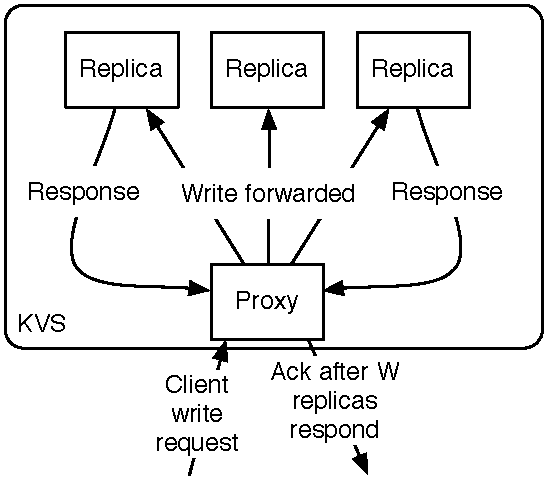
\includegraphics[width=.8\columnwidth]{figs/dynamo-quorum.pdf}
\caption{Diagram of control flow for client write to Dynamo-style
  quorum.  Here, $N=3$, $W=2$. The client write is handled by a
  coordinator node and sent to all replicas. The write succeeds when
  $W$ replicas respond.  Note that the coordinator is possibly a
  replica as well, invoking a local write.}
\label{fig:dynamo-quorum}
\end{figure}

Many Dynamo-style systems also support additional anti-entropy
processes~\cite{nosql}.  One common feature is called \textit{read
  repair}~\cite{dynamo}.  When a read coordinator receives multiple
versions of a data item from different replicas in response to a read
request, it will attempt to (asynchronously) update the out-of-date
replicas with the most recent version.  The effect of read repair on
version drift between replicas is perhaps unsurprisingly dependent on
the read rate.  The original Dynamo paper used Merkle trees to
summarize and exchange data contents between replicas as a means of
secondary anti-entropy (after the initial write to $N$ replicas).
While open source Dynamo-style systems use Merkle trees, not all
actively employ them in gossip-based anti-entropy.  For example,
Cassandra only executes Merkle tree anti-entropy when it is manually
requested (e.g., \texttt{nodetool repair})~\cite{cassandra-merkle}.

There are significant differences between data systems in the wild and
the theory describing quorum operation.  First, replication factors
for distributed data systems are relatively low.  Typical replication
factors are between one and three, however the systems literature has
discussed replication up to a factor of 10~\cite{chain-replication}.
Second, (in the absence of failure), in Dynamo-style partial quorums,
the write quorum size increases even after the operation returns,
growing via anti-entropy.  Moreover, read requests are sent to all
replicas, however only the first $R$ responses are considered.  As a
matter of nomenclature (and to disambiguate against dynamic quorum
membership protocols), we will refer to these systems as
\textit{expanding partial quorum systems}.  Third, as in much of the
practical literature, practitioners largely focus on fail-stop failure
modes instead of Byzantine failure~\cite{birman-byzantine}.
Following standard practice, we do not consider Byzantine failure.

\section{Probabilistically Bounded\\Staleness}
\label{sec:pbs}

In this section, we introduce the theory of Probabilistically Bounded
Staleness to describe the consistency provided by existing eventually
consistent data stores.  PBS extends prior work on
probabilistic quorums by accounting for staleness of both versions and
across time.  We introduce the notions of PBS $k$-staleness, which
stochastically limit the staleness of versions returned by read
quorums, PBS $t$-visibility, which stochastically bounds the time
before a committed version appears to readers, and PBS $<k,
t>$-quorums, a combination of the two prior models.


Practical concerns guide the following theoretical contributions.  We
begin by considering a model without anti-entropic processes.
Accordingly, we assume that $W$ ($R$) of $N$ replicas are randomly
selected for each write (read) operation.  We consider a write
``committed'' once it has reached at least $W$ replicas and $W$ replicas
respond.  Similarly, we consider fixed $W$, $R$ and $N$ across
multiple operations. Subsequently, we expand our model to consider
write propagation and time-varying $W$ sizes, as is typically the case
in practice.  In this section, we discuss anti-entropy in general,
however we model Dynamo-style quorums in Section
\ref{sec:dynamo}. We discuss further refinements to our
assumptions in Section \ref{sec:discussion}.

\subsection{PBS $k$-staleness}

Probabilistic quorums allow us to determine the probability of
returning the most recent value written to the database, but do not
tell us what happens when the most recent value is not returned.
Here, we determine the probability of returning a value within a
bounded number of versions.  In the following model, we non-expanding 
write quorums (no anti-entropy) and compose multiple independent write
quorums to model the probable overlap of $k$ independent write sets.
\begin{definition}
A quorum system obeys \textit{PBS $k$-staleness consistency} if, with
probability $1-p_{staler}$, at least one value in any read quorum will
have been committed no later than $k$ versions after the latest committed
version when the read begins.
\end{definition}
Versions whose writes that are not yet committed (in-flight) may be
returned by a read in this formulation of probabilistic $k$-quorums
(see Figure \ref{fig:timelines}A).  The $k$-quorum literature defines
these as $k$-regular semantics~\cite{non-strict}.

\begin{figure}
\centering
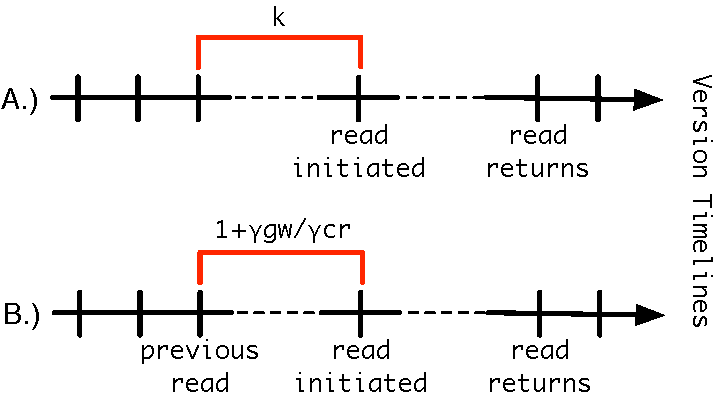
\includegraphics[width=\columnwidth]{figs/timelines.pdf}
\caption{Possible versions returned by read operations under
  PBS $k$-staleness (A) and PBS monotonic reads (B). In
  $k$-consistency, the read operation will return a version no later
  than $k$ versions older than the last committed value when it
  started; more versions may be committed during the read and may be
  returned.  In monotonic reads consistency, the staleness depends on
  the number of versions committed since the time the client last
  completed a read.  This is determined by the proportion of client's
  reads to the number of writes committed to the object.}
\label{fig:timelines}
\end{figure}

The probability of returning a version of a key within the last $k$
versions committed is equivalent to intersecting one of $k$
independent write quorums.  Given a probability of intersecting with a
single write quorum $p$, the probability of intersecting one of $k$
independent quorums is $p^k$.  Accordingly, if we assume a random
quorum choice, the probability of non-intersection is simply Equation
\ref{eq:prob-strict} exponentiated by $k$:
\begin{equation}
\label{eq:k-consistency}
p_{staler} = \left(\frac{{N-W \choose R}}{{N \choose R}}\right)^k
\end{equation}

For the $N=3, R=W=1$ case, this means that the probability of
returning a version within $2$ versions is $.\overline{5}$, within $3$
versions $.\overline{703}$, and within $5$ versions $> .868$, and $10$
versions $>.98$.  With $N=3, R=1, W=2$ (alternatively, $R=2, W=1$),
these probabilities increase: $k=1 \rightarrow
.\overline{6}$, $k=2 \rightarrow .\overline{8}, k=5 \rightarrow >
.995$.

This analytical closed form solution holds for quorums that do not
change size over time.  For quorums with asynchronously propagating
writes, this solution is an upper bound on the probability of
staleness.  We discuss the \textit{load} improvements offered by PBS
$k$-staleness as discussed in quorum system literature in Appendix A.

\subsection{PBS Monotonic Reads}

With additional information, we can use PBS $k$-quorums to predict
whether a client will ever read staler data than it has already read.
This property, known as \textit{monotonic reads} consistency is a
well-known session guarantee~\cite{sessionguarantees}.

\begin{definition}
\label{def:prob-mr}
A quorum system obeys \textit{PBS monotonic reads consistency} if,
with probability at least $1-p_{staler}$, at least one value in any
read quorum returns the same version or a newer version than the last
version that a client has previously read, where versions are defined
over the global commit ordering.
\end{definition}

To guarantee that a client sees monotonically increasing versions, it
can continue to contact the same replica~\cite{vogels-defs}.  However,
this is insufficient to guarantee strict monotonic reads (where the
client reads strictly newer data if it exists in the system).
Definition~\ref{def:prob-mr} can be adapted to accommodate strict
monotonic reads by requiring that, if a more recent data version is
available, it is returned.

We observe that monotonic reads is a special case of PBS $k$-quorums
(see Figure~\ref{fig:timelines}B), where $k$ is determined by a
client's rate of reads from a data item ($\gamma_{cr}$) and the
global, system-wide rate of writes to the same data item
($\gamma_{gw}$).  If we know these rates exactly, the number of
versions between client reads is $\frac{\gamma_{gw}}{\gamma_{cr}}$, as
shown in Figure \ref{fig:timelines}B.  We can calculate the
probability of probabilistic monotonic reads as a special case of
$k$-staleness where $k=1+\frac{\gamma_{gw}}{\gamma_{cr}}$.  For
example, extending the example in Equation \ref{eq:k-consistency}:

\begin{equation}
\label{eq:prob-mr}
p_{staler} = \left(\frac{{N-W \choose R}}{{N \choose R}}\right)^{1+\gamma_{gw}/\gamma_{cr}}
\end{equation}
For strict monotonic reads, where we cannot read the version we have
previously read (assuming there are newer versions in the database),
we exponentiate where $k=\frac{\gamma_{gw}}{\gamma_{cr}}$.  

In practice, we may not know these exact rates, but, by measuring
their distribution, we can calculate an expected ratio that we can
integrate into these calculations.  By performing appropriate
admission control, operators can control these rates to achieve
monotonic reads guarantees.

\subsection{PBS $t$-visibility}
\label{sec:tvis}


Until now, we have considered only quorums that do not grow over time.
However, as we discussed in Section \ref{sec:practice}, modern quorum
systems in practice asynchronously propagate writes to quorum system
members over time.  This process is commonly known as
anti-entropy~\cite{antientropy}.  For generality, in this section, we
will discuss general anti-entropy models. However, we explicitly model
the Dynamo-style anti-entropy mechanism in Section \ref{sec:dynamo}.

PBS $t$-visibility models the probability of inconsistency, accounting
for the propagation of writes across wall-clock time such that the set
of replicas with a given version of the data (or later) grows over
time.  Node failures shrink this set and can be incorporated into this
model, but we do not consider them here.  Intuitively, $t$-visibility
captures the possibility that a reader will observe a write $t$
seconds after it commits.  Recall that we consider in-flight
writes---which are more recent than the last committed version---as
non-stale.

\begin{definition}
A quorum system obeys \textit{PBS $t$-visibility consistency} if, with
probability $1-p_{staler}$, any read quorum started at least $t$ units
of time after the last version committed returns at least one value
that is at least as recent as the last version committed when the read
began (and may not be committed yet).
\end{definition}

We denote the cumulative density function describing the number
of replicas $\mathcal{W}$ that have a particular version $v$ (or a
version committed after $v$) $t$ seconds after committing as
$P_w(\mathcal{W}, t)$.

By definition, $P_w(c,0) = 1$ $\forall c \in [0, w]$.  Intuitively, at
commit time, $W$ replicas will have the value, so the probability that
zero to $W$ replicas have the value immediately after commit is
exactly $1$.  We can model the probability of PBS $t$-visibility for
an interval $t$ by summing the conditional probabilities of each
possible $\mathcal{W}$:

\begin{equation}
\label{eq:tv-instantreads}
p_{staler} = \frac{{N-W \choose N}}{{N \choose R}}+\sum_{c\in(W, N]} \frac{{N-c \choose N}}{{N \choose R}}\cdot [P_w(c+1, t)-P_w(c,t)]
\end{equation}

However, the above equation assumes reads occur instantaneously and
writes commit immediately after $W$ replicas have the version (i.e.,
there is no delay back to a coordinating node).  In the real world,
writes need to be acknowledged and reads must be sent to replicas.
Therefore more time will elapse between the time $W$ of $N$ replicas
have a version and $t$.  Accordingly,
Equation~\ref{eq:tv-instantreads} is a conservative upper bound on
$t$-staleness.  Additionally, one can model both transient and
permanent failures by increasing the tail probabilities for operation
latencies.

In practice, $P_w$ depends on the anti-entropy protocols and the
expected latency of operations and can be approximated (Section
\ref{sec:dynamo}) or measured online.  For this reason, the load of a
PBS $t$-visible quorum system depends on write propagation and is
difficult to determine for general-purpose dynamic quorums.


\subsection{PBS $\langle k, t
  \rangle$-staleness Consistency}

We can combine the previous models to combine both versioned and
real-time staleness metrics to answer questions of the following form:
what is the probability that a read will return a value no older than
$k$ versions stale if the last write committed no sooner than $t$ seconds
ago?
\begin{definition}
A quorum system obeys \textit{probabilistic $\langle k, t
  \rangle$-staleness consistency} if, with probability $1-p_{staler}$, at
least one value in any read quorum will have been committed no later
than $k$ versions after the latest committed version when the read
begins, provided the read begins $t$ units of time after the previous
$k$ versions commit.
\end{definition}
The definition of $p_{staler}$ follows from the prior definitions:
\begin{equation}
p_{staler} = (\frac{{N-W \choose R}}{{N \choose R}}+\sum_{c\in[W, N)} \frac{{N-c \choose R}}{{N \choose R}} \cdot [P_w(c+1, t)-P_w(c,t)])^k
\end{equation}
In this equation, in addition to (again) assuming instantaneous reads,
we also assume the pathological case where the last $k$ writes all
occurred at the same time.  This is not likely in practice, so if we
can determine the time since commit for the last $k$ writes, we can
improve this staleness bound by considering each quorum's $p_{staler}$
at $RT=t$ separately.  However, this equation provides a conservative
upper bound on $p_{staler}$.

Note that the prior definitions of consistency are encapsulated by
probabilistic $\langle k, t \rangle$-quorum consistency. probabilistic
$k$-quorum consistency is simply probabilistic $\langle k, 0
\rangle$-quorum consistency, probabilistic monotonic reads consistency
is $\langle 1+\frac{\gamma_{gw}}{\gamma_{cr}}, 0 \rangle$-quorum
consistency, and $t$-visibility is $\langle 0, t \rangle$-quorum
consistency.

In practice, we believe it is easier to reason about staleness of
versions or staleness in terms of real time but not both together.
Accordingly, having derived a closed-form model for $k$-visibility, in
the remainder of this paper, we focus mainly on deriving specific models
for $t$-visibility.

\section{Dynamo-style $t$-visibility}
\label{sec:dynamo}

We have formulated a closed-form analytical model for $k$-staleness,
but $t$-visibility is dependent on both the distributed quorum
execution algorithm and the anti-entropy protocols employed by a data
storage system.  In this section, we discuss PBS $t$-visibility in the
context of Dynamo-style data storage systems.  We describe how to
model the probability of staleness in these systems and how to
asynchronously detect staleness.

\subsection{Inconsistency in Dynamo: WARS Model}

Dynamo-style quorum systems are inconsistent as a result of read and
write message reordering.  Reads and writes are sent to all quorum
members, so the staleness under normal operation results only when one
of the first $R$ read responses beat the last committed write to its
corresponding replica.  To demonstrate this phenomenon, we introduce a
model of Dynamo operation which, for convenience, we will call \textit{WARS} .

We illustrate \textit{WARS} in Figure~\ref{fig:dynamo-diagram}, a space-time
diagram for messages between a coordinator and a single replica for a
write followed by a read $t$ seconds after the write commits.
This $t$ corresponds to the $t$ in $t$-visibility.

\begin{figure}
\centering
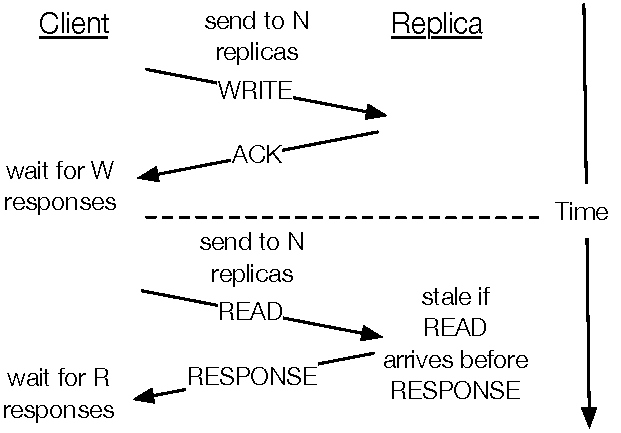
\includegraphics[width=.8\columnwidth]{figs/dynamostale.pdf}
\caption{The \textit{WARS}  model for message ordering in Dynamo describes the
  message flow between a coordinator and a single replica for a write
  followed by a read $t$ seconds after commit.  Note that, in an $N$
  replica system, this message flow is replicated $N$ times between
  the coordinator and $N$ replicas.  Note that the read and write may be handled by different coordinators.}
\label{fig:dynamo-diagram}
\end{figure}

For a write, the coordinator sends $N$ messages, one to each
replica. The message from coordinator to replica containing the
version to be written is delayed by a value chosen from distribution
\texttt{W}.  The coordinator waits for $W$ responses from the replicas
before it can consider the version committed.  Each response is delayed by
a value chosen from the distribution \texttt{A}.

For a read, the coordinator sends $N$ messages, one to each replica.
The message from coordinator to replica containing the read request is
delayed by a value chosen from distribution \texttt{R}.  The
coordinator waits for $R$ responses from the replicas before returning
the most recent value it recieves.  Each read response is delayed by a
value chosen from the distribution \texttt{S}.

In the absence of additional anti-entropic processes, the coordinator
will return stale data if all $R$ of the $N$ responses received before
the read returns reached their respective replicas before the
respective message delayed by \texttt{W} does.  When $R$$+$$W$$>$$N$,
this is impossible.  However, under partial quorums (when
$R$$+$$W$$\leq$$N$), this depends on the latency distributions.  If we
denote the commit time as $w_t$, to observe staleness, $r+w_t < w$ for
$r$ chosen from \texttt{R} and $w$ chosen from \texttt{W}.  Writes
have time to propagate to additional replicas both while the
coordinator waits for all required acknowledgments (\texttt{A}) and as
read requests are subsequently sent (\texttt{R}).  Similarly, read
responses are further delayed in transit (\texttt{S}) back to the read
coordinator, inducing further possibility of reordering.
Qualitatively, longer write tails and faster reads increase the chance
of staleness due to the possibility of reordering.

Depending on which coordinator a client contacts, some reads and
writes may be served locally.  In this case, subject to local query
processing delays, a read or write to $R$ or $W$ nodes is behaves like
a read or write to $R-1$ or $W-1$ nodes, respectively.  Although we do
not do so, \textit{WARS} can be adopted to handle local reads and
writes.  Proxying reads is conservative, while proxying writes may
increase staleness.

An individual client will likely incur additional time between its
reads and writes due to latency required to contact the data store.
An individual making requests to a web service using his or her
browser will likely incur tens or hundreds of milliseconds of delay
between requests.  We consider global read and write traffic in our
analysis and do not consider this delay here, but this delay is useful
to consider in practical scenarios.

\textit{WARS} considers the effect of message sending, delays, and
reception, but this represents a daunting analytical formulation.  The
commit time represents an order statistic dependent on both \texttt{W}
and \texttt{A}. \begin{comment}{\color{red}: Peter A ``confused''}\end{comment}  Furthermore, message reordering is dependent on the
commit time.  The probability that the $i$th returned read message
observes reordering is both an order statistic dependent on $W$ and
$A$, and, between $i$, the probabilities are dependent.  The expected
read and write latencies can be computed using simple order statistics
if one makes independence assumptions about the distributions in
\textit{WARS} .  However, a concise, closed form for the probability
of inconsistency eludes us.  Dynamo is simple to reason about and
program, but difficult to analyze in closed form.  As we discuss in
Section~\ref{sec:dynamoeval}, we explore \textit{WARS} using Monte
Carlo analysis, which suffices for our purposes in practice and, from
a practical perspective, is relatively easier to implement.

\subsection{Additional Anti-entropy}

As we discussed in Section~\ref{sec:practice}, anti-entropic processes
anti-entropic processes decrease the probability of staleness by
further propagating versions between members.  In addition to
write-all semantics, Dynamo employs read repair and Merkle tree
exhange. However, both of these processes are rate dependent: read
repair effects depend on the rate of reads, and Merkle tree exchange effects
(and, more generally, the efficacy most anti-entropy protocols) depend on
the rate of exchange.  \textit{WARS} is read rate independent but is
affected by the write rate.  If multiple writes overlap, that is, have
overlapping periods where they are in-flight but are not committed,
the probability of inconsistency decreases.  Intuitively, this is
because overlapping writes results in increased chance that a
client reads as-yet-uncommitted data.  Accordingly, because \textit{WARS} does
not capture read repair or Merkle tree exchange, it
represents a lower bound for Dynamo-style operation for the sake of
simplicity of analysis.  In practice, versions may be fresher than predicted.\begin{comment} {\color{red} Peter A: more general}\end{comment}

In the presence of multiple concurrent writes (or even periodic
writes), $t$-visibility time is bounded by the time between writes.
Intuitively, if two writes to a key are spaced $m$ milliseconds apart,
then the $t$-visibility of the first write for $t > m+k$ milliseconds
for $k >0$ is undefined; it is no longer the last committed version.
Accordingly, practical $\langle k, t \rangle$-staleness requires
assumptions regarding the write arrival rate (instead of
pessimistically assuming that all $k$ writes finished simultaneously
$t$ seconds ago).

\subsection{Asynchronous Staleness Detection}

Even if a system provides an extremely high probability of
consistency, it is may be useful if applications can be notified when
data returned is inconsistent, or staler than expected.  The Dynamo
model is naturally equipped for staleness detection.

Knowing whether a response is stale at read time requires strong
consistency.  Assume staleness detection did not require strong
consistency.  By checking all possible values in the domain against
the staleness detector, we could determine the consistent value.
Conversely, if we do not have strong consistency, then we cannot
determine the last committed version. However, we \textit{can}
determine staleness asynchronously.  Asynchronous staleness detection
allows speculative execution~\cite{nsdispeculation} if a program
contains appropriate compensation logic.

We first consider a staleness detector that provides false positives.
Recall that, in a Dynamo-style system, we wait for $R$ of $N$ replies
before returning a value.  The remaining $N-R$ replicas will still
reply to the read coordinator.  Instead of dropping these messages,
the coordinator can compare them to the version it returned.  If there
is a mismatch, then either the coordinator returned stale data, there
are in-flight writes in the system, or additional versions committed
after the read. The latter two cases, relating to data committed after
the response was initiated, lead to false positives.  We define
staleness according to the last committed write when the read began,
so versions written after the last committed version do not
technically constitute stale reads.  Notifying clients of newer
versions of a data item is not necessarily bad but may be unnecessary
and violates our staleness semantics.  Note that this detector does
not require modifications to the Dynamo protocol and is similar to the
read-repair process.

To eliminate false positives, we need to determine the total,
system-wide commit ordering of writes. Recall that replicas are
unaware of the commit time for each version; commits occur after $W$
replicas respond and the version stamps that replicas store are not
updated after commit.  Establishing a total ordering is a well-known
distributed systems problem that could be accomplished in Dynamo using
a centralized service~\cite{zookeeper} or using distributed
consensus~\cite{paxos}.  Eliminating false positives requires
modifications to the Dynamo protocol but is definitely feasible.

While this discussion has been couched in the terms of strong
consistency, it is easily extended to PBS $k$-staleness and PBS
$\langle k, t \rangle$-staleness.

\section{Evaluating Dynamo $t$-visibility}
\label{sec:dynamoeval}

As discussed in Section~\ref{sec:tvis}, PBS $t$-visibility depends on
the propagation of reads and writes throughout a system.  We
introduced the \textit{WARS}  model as a means of reasoning about
inconsistency in Dynamo-style quorum systems, but quantitative metrics
such as staleness observed in practice depend on each of \textit{WARS} 's
latency distributions.  In this section, we perform an analysis of
Dynamo-style $t$-visibility under several different assumptions.  We
use a mix of real-world experiments and Monte Carlo analyses
under distributions from production environments to better
understand how frequently ``eventually consistent'' means
``consistent'' and, more importantly, why.

Recall that PBS $k$-staleness is easily captured in closed form for
non-entropic quorums.  In practice, without anti-entropy, we observe
that their equations hold true.  However, in a system employing
anti-entropy, we cannot disentangle time and versions.  In this
section, we focus mainly on $t$-visibility but briefly describe some
$\langle k, t \rangle$-staleness results.

In this section, we focus on worst-case bounds for staleness.  While
we could improve the staleness results by considering additional
anti-entropic processes, we make the bare minimum of assumptions as
dictated by the \textit{WARS}  model.  Opting for conservative analyses
decreases the number of varibles in our experiments (each of which is
supported by empirical observations from practitioners) and increases
the applicability of these results.

\subsection{Monte Carlo Simulator}

We implemented \textit{WARS}  in a simple event-driven simulation environment.
Calculating $t$-visibility for a given value of $t$ is rather
straightforward: draw $N$ samples from \texttt{W}, \texttt{A},
\texttt{R}, and \texttt{S} at time $t$ (denote index $i$ as $[i]$), compute $w_t = \texttt{W}[W]+\texttt{A}[W]$, and check whether the
first $R$ samples of \texttt{R}, ordered by
$\texttt{R}[i]+\texttt{S}[i]$ obey $w_t+\texttt{R}[i] \leq
\texttt{W}[i]$.  This requires only a few lines of code.  Implementing
$\langle k, t \rangle$-staleness requires remembering write ordering
and history but is not difficult.

\subsection{Model Validation}

To validate \textit{WARS}  (and our subsequent analyses), we instrumented a
commercially available, open source Dynamo-style key-value store to
measure the staleness observed under partial quorum operation.
Unsurprisingly, our observations matched \textit{WARS}.

We modified Cassandra, a data store originally designed at Facebook,
which provides Dynamo-style partial quorum semantics, offering
per-request quorum sizes and a BigTable-like data
model~\cite{cassandra, cassandra-sigmod}.  Our changes to Cassandra were minimal:
we added support for partial quorums of size greater than
three---requiring changes to the wire protocol and request handling
code---and instrumented parts of the database to provide timing
information about reads and writes.  By analyzing Cassandra logs, we
were able to reconstruct the latency distributions of write requests,
write acknowledgements, read requests, and read responses.  We
disabled read repair because it is external to \textit{WARS}.

To provide a single point of order for the series of reads and writes
in the system, we used $N+1$ Cassandra nodes for each experiment
involving $N$ nodes.  After configuring the Cassandra schema, we
determined the node that did not store the data and sent all requests
through it, effectively creating a remote proxy.  \textit{WARS} is
more general than the specific proxy configuration, however using a
centralized proxy allows us to avoid most issues with clock skew
between replicas and rely less heavily on globally synchronized
clocks.

We ran Cassandra on a set of machines with 2.2GHz AMD Opteron 2214
dual-core SMT processors with 4GB of 667MHz DDR2 memory serving
in-memory data.  To test \textit{WARS}, we inserted monotonically
increasing version numbers to a single key, while five concurrent
processes read values measured the probability of staleness at every
millisecond.  We injected a set of delays into both the request and
response sending modules in Cassandra (we discuss a range of
distributions in Section~\ref{sec:latencies}) and measured the
probability of staleness.  Under the empirically-measured delay
distributions, our simulation was accurate for $t$-visibility for
$t\in\{1,\cdots,199\}$ with RMSE=0.0023\%.  This validates our Monte
Carlo analysis.

\subsection{Production Latency Distributions}
\label{sec:latencies}

\textit{WARS} depends only on latency distributions, and, rather than
conjecture as to what represents ``reasonable'' scenarios, we analyzed
production distributions from two internet-scale companies, LinkedIn
and Yammer.

LinkedIn~\cite{linkedin} is an online professional social network
claiming over 135 million members as of November
2011~\cite{linkedinmembers}. To handle highly available, low latency
data storage, engineers at LinkedIn built Voldemort, a Dynamo-style
quorum replicated key value store~\cite{voldemort, voldemortpub}.
Alex Feinberg, a lead engineer on Voldemort, graciously provided us
with latency distributions for a single node replaying peak load
traffic for the ``Who Viewed My Profile?'' data set on LinkedIn,
representing 60\% read and 40\% read-modify-write
traffic~\cite{feinbergpc} (Table~\ref{table:linkedin}).  Feinberg
reports that ``with spinning disks, we're largely IO bound and latency
is largely determined by the kind of disks we're using, data to memory
ratio and request distribution.  With [solid state drives (SSDs)],
we're CPU and/or network bound (depending on value size).''  As an
interesting aside, Feinberg also notes that ``maximum latency is
generally determined by [garbage collection] activity (rare, but
happens occasionally) and is within hundreds of milliseconds.''

\begin{table}
\centering
\begin{tabular}{|c|c|}
\hline
\%ile & Latency (ms) \\
\hline
\multicolumn{2}{|c|}{ 15,000 RPM SAS Disk}\\
\hline
Average & 4.85\\
95 & 15\\
99 & 25\\
\hline
\multicolumn{2}{|c|}{ Commodity SSD }\\
\hline
Average & 0.58 \\
95 & 1\\
99 & 2\\
\hline
\end{tabular}
\caption{LinkedIn Voldemort single-node production latencies.}
\label{table:linkedin}
\end{table}

Yammer is an online social network designed to provide enterprises
with private social networking capabilities.  As of December 2011,
Yammer claimed over 100,000 companies as customers~\cite{yammer}.
Yammer uses Basho's Riak, another open source Dynamo-style quorum
replicated database for client data~\cite{riak}.  Coda Hale,
infrastructure architect, and Ryan Kennedy, also of Yammer, presented
on their use of Riak including surprisingly in-depth performance
numbers in March 2011~\cite{riakyammer}.  Yammer provided us with more
detailed performance numbers for their application~\cite{codapc}
(Table~\ref{table:yammer}).  Hale noted that ``reads and writes have
radically different expected latencies, especially for Riak. Writes
don't return until the fsync returns, so while reads are often $<$
1ms, writes rarely are.''  As we will see, this has important
consequences for \textit{WARS}.  Although we do not model this
explicitly, Hale also notes that ``value size is also interesting. We
saw a big performance improvement by adding LZF compression to
values.''

\begin{table}
\centering
\begin{tabular}{|c|c|c|}
\hline
\%ile & Read Latency (ms) & Write Latency (ms)\\
\hline
Min & 1.55 & 1.68\\
50 & 3.75 & 5.73 \\
75 & 4.17 & 6.50\\
95 & 5.2 & 8.48\\
98 & 6.045 & 10.36 \\
99 & 6.59 & 131.73\\
99.9 & 32.89 & 435.83\\
Max & 2979.85 &  4465.28 \\
\hline
Mean & 9.23 & 8.62 \\
Std. Dev. & 83.93 & 26.10\\
\hline
Mean Rate & 718.18 gets/s & 45.65 puts/s\\
\hline
\end{tabular}
\caption{Yammer Riak $N$$=$$3$, $R$$=$$2$, $W$$=$$2$ production latencies.}
\label{table:yammer}
\end{table}

\subsection{Production Latency Model Fitting}

While insights from production data are invaluable, they are
underspecified for \textit{WARS}.  First, they are summary statistics,
so we need to calculate the underlying distribution.  More
importantly, the operation latencies represent round-trip times, while
\textit{WARS} requires the constituent one-way latencies for reads and
writes.  Accordingly, to derive
\texttt{W},\texttt{A},\texttt{R},\texttt{S} for each configuration, we
made a series of assumptions.  These assumptions are imperfect, and do
not perfectly mirror the real world.  As we demonstrated in our
Cassandra experiments, these latency distributions are easily
collected.  However, because they are not currently collected in
practice, we must do our best to fill in the gaps.  Without additional
data on the latency required to read multiple replicas, we assume that
each latency distribution is independently, identically distributed.
We believe that these assumptions are justified given the advantage of
production data over synthetic distributions.

LinkedIn provided two latency distributions, which we denote
\texttt{LNKD-SSD} and \texttt{LNKD-DISK} for the SSD and spinning
disks, respectively.  As previously discussed, when running on SSDs,
Voldemort is largely network and CPU bound.  Accordingly, we assumed
that read and write operations took equivalent amounts of time and, to
split the remaining time, we focused on the network-bound case and
assumed that one-way trips were symmetric
(\texttt{W}=\texttt{A}=\texttt{R}=\texttt{S}).  This allowed us to
derive \texttt{LNKD-SSD}.  For \texttt{LNKD-DISK}, Feinberg mentioned
that Voldemort performs at least one read before every write (average
of 1 seek, between 1-3 seeks), and writes to the BerkeleyDB Java
Edition backend are flushed every 30 seconds or 20
megabytes---whichever comes first.  Accordingly, we kept the same
\texttt{A}=\texttt{R}=\texttt{S} as in \texttt{LNKD-SSD} but
calculated \texttt{W} separately.  

\begin{table}
\centering
\begin{tabular}{|c|r|}
\hline
\multirow{4}{*}{\texttt{LNKD-SSD}} & \multicolumn{1}{|l|}{$\texttt{W} = \texttt{A}= \texttt{R} = \texttt{S}:$} \\
& 8.78\%: Exponential, $\lambda = 1.66$ \\
& 91.22\%: Pareto, $x_m=.235, \alpha=10$\\
& N-RMSE: .55\%\\\hline
\multirow{4}{*}{\texttt{LNKD-DISK}} & \multicolumn{1}{|l|}{$\texttt{A}= \texttt{R} = \texttt{S}: \texttt{LNKD-SSD}$}\\\cline{2-2}
& \multicolumn{1}{|l|}{\texttt{W}:}\\
& \hfill 62\%: Exponential, $\lambda = .183$ \\
& 38\%: Pareto, $x_m=1.05, \alpha=1.51$\\
& N-RMSE: .26\%\\
\hline
\multirow{8}{*}{\texttt{YMMR}} & \multicolumn{1}{|l|}{\texttt{W}:} \\
& 6.1\%: Exponential, $\lambda = .0028$ \\
& 93.9\%: Pareto, $x_m=3, \alpha=3.35$\\
& N-RMSE: 1.84\%\\\cline{2-2}
& \multicolumn{1}{|l|}{$\texttt{A}= \texttt{R} = \texttt{S}:$}\\
& 1.8\%: Exponential, $\lambda=.0217$\\
& 98.2\%: Pareto, $x_m=1.5, \alpha=3.8$\\
& N-RMSE: .06\%\\
\hline
\end{tabular}
\caption{Distribution fits for production latency distributions.}
\label{table:fits}
\end{table}


Yammer provided distributions for a single configuration but separated
read from write latencies, which we denote \texttt{YMMR}.  Using our
IID assumptions, we fit single-node latency distributions to the
provided distributions, again assuming symmetric \texttt{A},
\texttt{R}, and \texttt{S}.  The data fit a Pareto distribution with a
long exponential tail.  At the $98$th percentile, the write
distribution takes a sharp turn.  Fitting the data closely resulted in
an extremely long tail, with $99.99+$th percentile writes requiring
tens of seconds, much higher than Yammer specified.  Accordingly, we
fit the $98$th percentile knee conservatively---without the $98$th
percentile, the write fit N-RMSE is .104\%.


\begin{figure*}[t!]
\centering
\subfigure{
\includegraphics[width=\columnwidth]{figs/latlegend.pdf}}\\[-1mm]
\subfigure{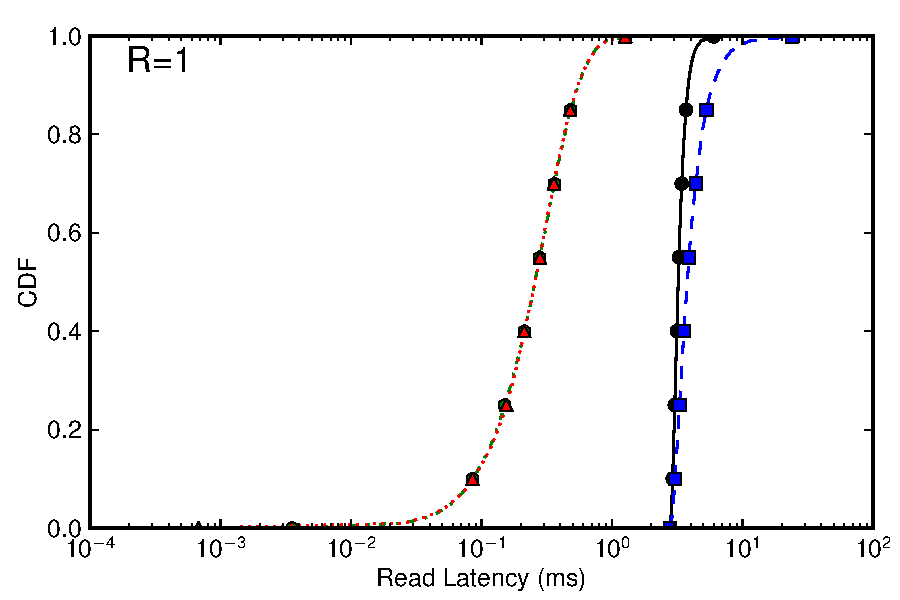
\includegraphics[width=.6\columnwidth]{figs/readlats-1.pdf}}
\subfigure{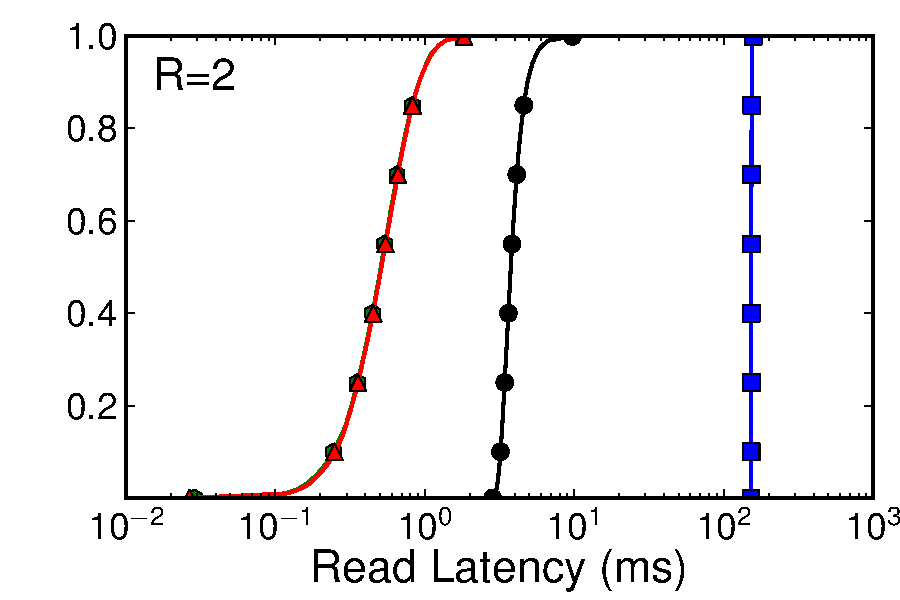
\includegraphics[width=.6\columnwidth]{figs/readlats-2.pdf}}
\subfigure{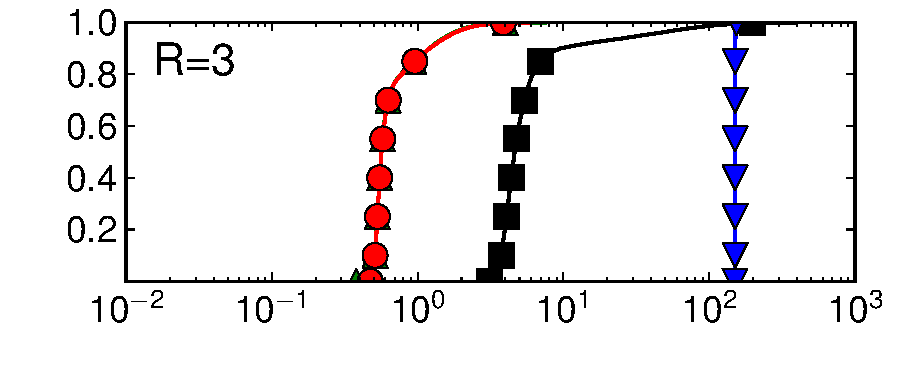
\includegraphics[width=.6\columnwidth]{figs/readlats-3.pdf}}
\subfigure{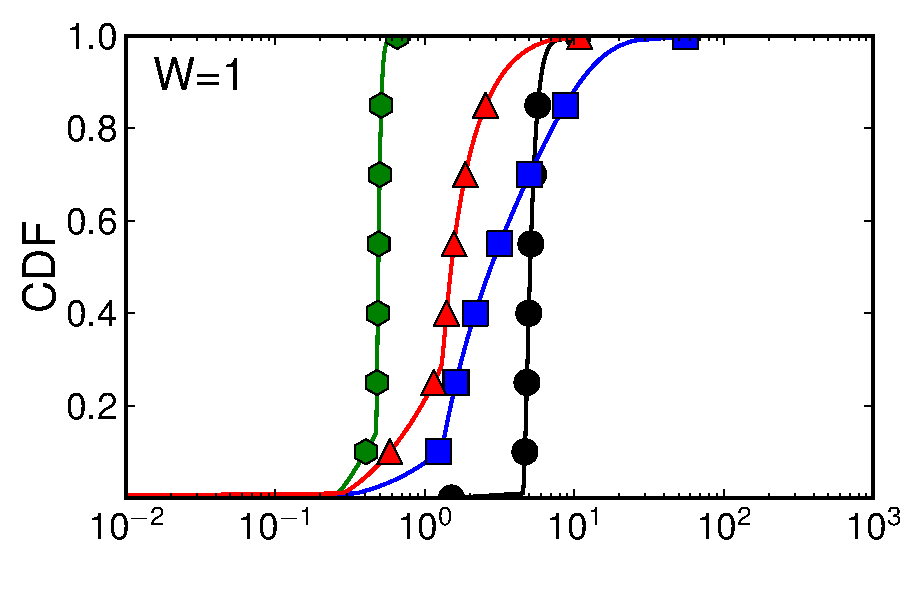
\includegraphics[width=.6\columnwidth]{figs/writelats-1.pdf}}
\subfigure{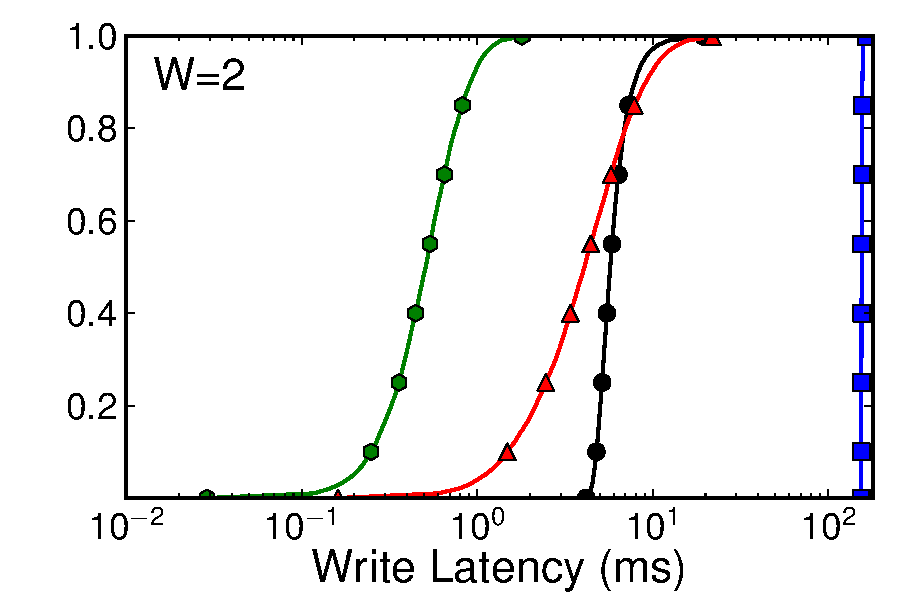
\includegraphics[width=.6\columnwidth]{figs/writelats-2.pdf}}
\subfigure{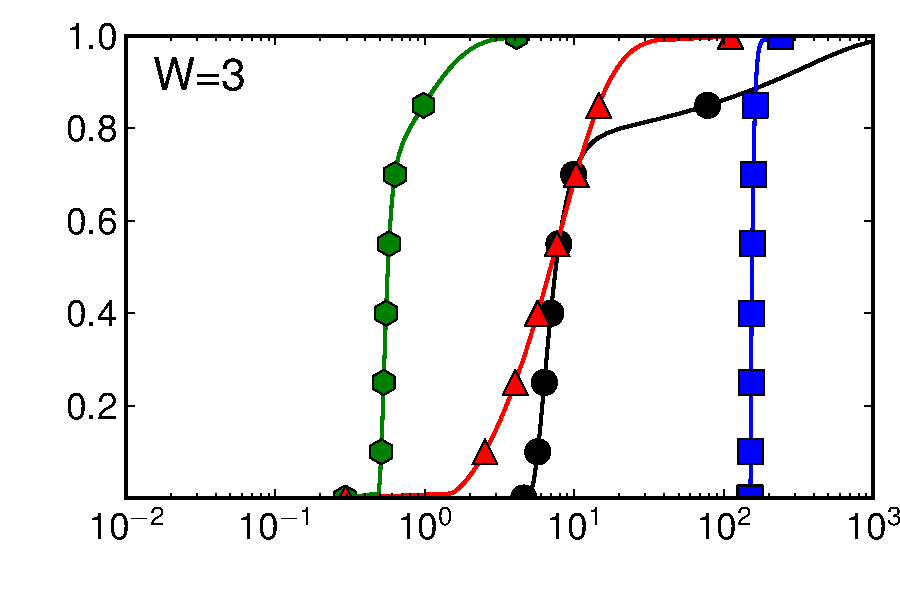
\includegraphics[width=.6\columnwidth]{figs/writelats-3.pdf}}
\caption{Read and write operation latency for \textit{WARS} latencies fitted
  to production datasets for $N$$=$$3$.}
\label{fig:latencies}
\end{figure*}

Finally, we simulated a normal-case WAN replication scenario,
\texttt{WAN}.  Reads and writes are routed to random data centers,
and, accordingly, one replica operation commits quickly while the
others are routed remotely.  We delay remote operations and responses
by 75ms and apply \texttt{LNKD-DISK} delays once the operation reaches its
target data center, in accordance with a near-worst-case
multi-continent WAN network delay~\cite{dean-keynote}.

We show the parameters for each distribution in
Table~\ref{table:fits}. We plot each fitted distribution in
Figure~\ref{fig:latencies}.  Note that for $R$, $W$ of one,
\texttt{LNKD-DISK} is not equivalent to \texttt{WAN}.  This is
because, in \texttt{LNKD-DISK}, we only have to wait for the first of
$N$ local reads (writes) to return, whereas there is only one local
read (write) for \texttt{WAN}, and all other read (write) requests will
be delayed at least 150ms.

\subsection{Observed $t$-visibility}

We measured the $t$-visibility for each distribution
(Figure~\ref{fig:tvis}).  We simulated reads
after each of 10,000 non-overlapping writes staggered by time
and calculated the probability of consistency, or 
$t$-visibility across time.

As our qualitative \textit{WARS} analysis predicted, the probability
of consistency was largely dependent on the write tail size.
Immediately after write commit, with $N$$=$$3$, $R$$=$$W$$=$$1$,
\texttt{YMMR} had a $89.3\%$ chance of consistency, \texttt{LNKD-SSD}
had a $97.5\%$ chance, and \texttt{LNKD-DISK} had a $43.9\%$ chance.
Ten milliseconds after write commit, \texttt{YMMR} had a $93.9\%$
chance of consistency, \texttt{LNKD-SSD} had a $100\%$ chance, and
\texttt{LNKD-DISK} had a $92.5\%$ chance.  \texttt{YMMR}'s tall body
but long tail limited its probability increase, and only reached
$99.9\%$ consistency 1364 ms after writing.  \texttt{LNKD-SSD}'s reads
raced its writes immediately after commit, but, one millisecond after
the write, the chance of a read round-trip time plus one millisecond
beating its write was almost eliminated.  \texttt{LNKD-DISK} had the
the longest body of these three distributions but reached $99.9\%$
confidence after 45.5 ms (having a shorter tail than \texttt{YMMR}).  As
expected, \texttt{WAN} observed poor chances of consistency until
after the 75 milliseconds passed; unless a reader read from the same
datacenter in which the last write committed, it had to wait for the
long propagation to observe the most recent value.

\begin{figure*}
\centering
\subfigure{
\includegraphics[width=\columnwidth]{figs/latlegend.pdf}}\\[-1mm]
\subfigure{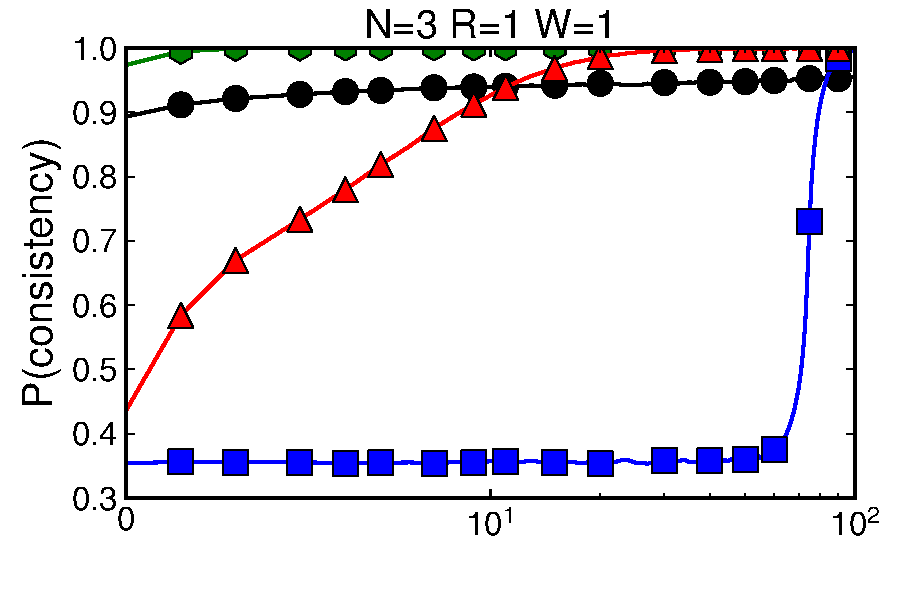
\includegraphics[width=.65\columnwidth]{figs/tstales-3N1R1W.pdf}}
\subfigure{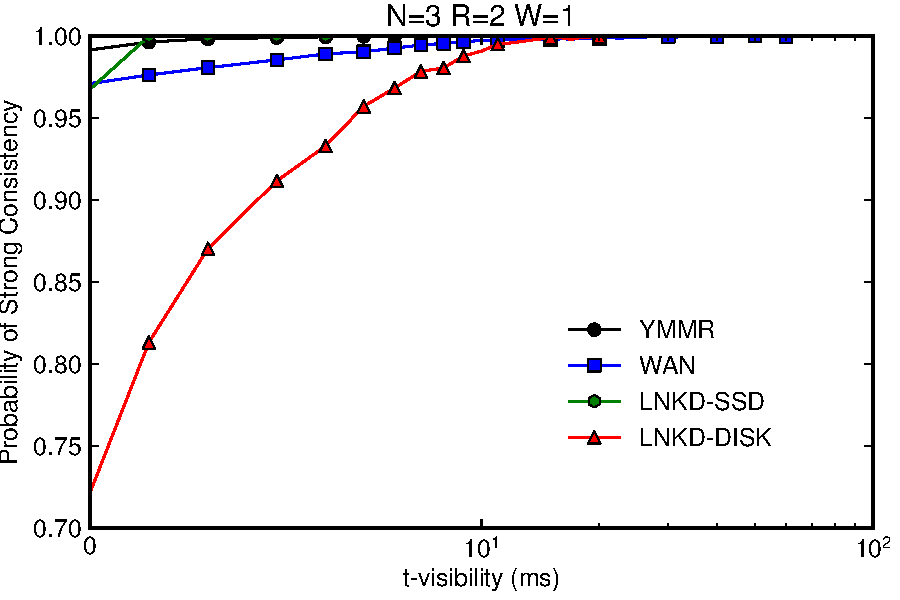
\includegraphics[width=.65\columnwidth]{figs/tstales-3N2R1W.pdf}}
\subfigure{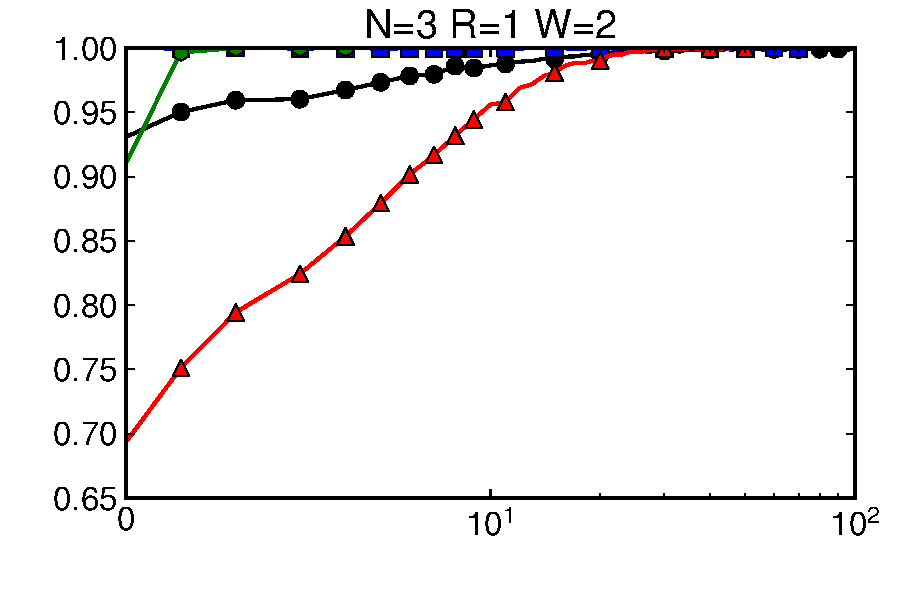
\includegraphics[width=.65\columnwidth]{figs/tstales-3N1R2W.pdf}}
\caption{$t$-visibility for production operation latencies.}
\label{fig:tvis}
\end{figure*}

\subsection{Latency Tail Effects}

%the ratio of \texttt{W} to \texttt{A}=\texttt{R}=\texttt{S} and swept
%a range of exp 
To better understand the impact of write tail latency on
$t$-staleness, we swept a range of exponential distributions, fixing
\texttt{A}=\texttt{R}=\texttt{S} and varying \texttt{W}.  The results,
shown in Figure~\ref{fig:varydelay}, indicate that probability of
consistency is largely influenced by the write latency. When the mean
of \texttt{W} ($.25$ms) is one-fourth the mean of
\texttt{A}=\texttt{R}=\texttt{S}, we observe a $94\%$ chance of
consistency immediately after the write and $99.9\%$ chance after 1ms.
However, when the mean of \texttt{W} ($10$ms) is ten times the mean of
\texttt{A}=\texttt{R}=\texttt{S}, we observe a $41\%$ chance of
consistency immediately after write and a $99.9\%$ chance of
consistency after $65$ ms. This result corroborates our earlier
observation that employing SSDs lowers the write latency and results
in lower $t$-visibility when compared to using disks.  More generally,
this result suggests that instead of increasing read and write quorum
sizes to decrease $t$-visibility, operators could chose to lower
(relative) \texttt{W} latencies.  This is achievable through hardware
configurations or by delay read latencies.  However, this latter
option is potentially problematic for read-heavy workloads and
introduces queuing effects for reads and writes.

\begin{figure}
\centering
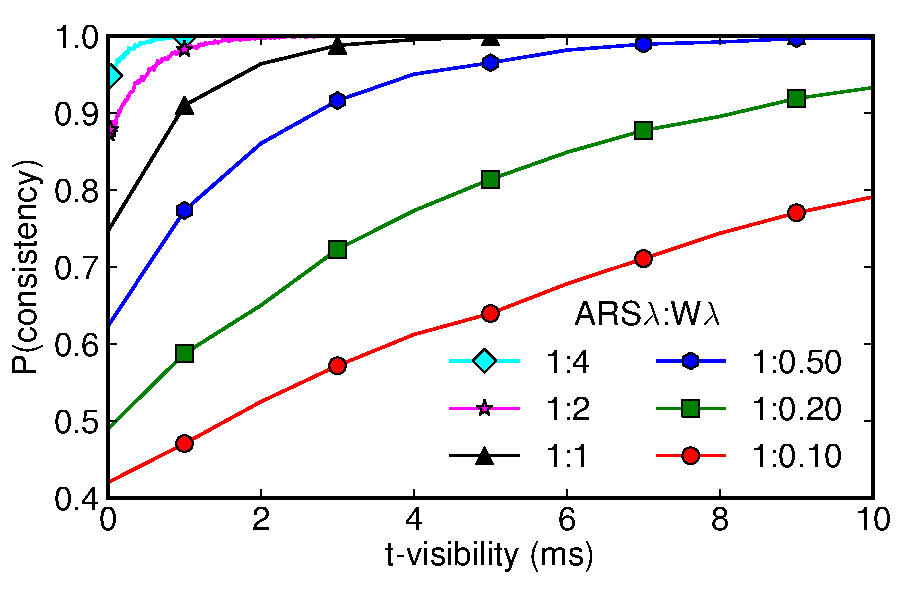
\includegraphics[width=.85\columnwidth]{figs/rwratio.pdf}
\caption{$t$-visibility for $N$$=$$3$, $R$$=$$W$$=$$1$ varying \texttt{W} and \texttt{A}=\texttt{R}=\texttt{S} exponentially distributed delays.  Mean latency is $1/\lambda$.}
\label{fig:varydelay}
\end{figure}

\subsection{Replica Size}

We consider how changing the number of replicas (N) affects
$t$-visibility while maintaining $R$$=$$W$$=$$1$. The results shown in
Figure~\ref{fig:varyn} show that the probability of consistency
immediately after write commit decreases as $N$ increases.  However,
at the tail, the $t$-visibility for increased replica sizes is
surprisingly close.  For example, the \texttt{LNKD-DISK} latency
distribution, the $t$-visibility at $99.9\%$ probability of
consistency ranges from $45.3$ ms for 2 replicas to $53.7$ ms for 10
replicas.  This implies that even if we choose to maintain a large
number of replicas for availability or better performance, the
$t$-visibility staleness will still converge relatively quickly for large $t$
grows. We believe the difference is larger due to the longer tail in
the write latency distribution.

\begin{figure*}
\centering
\subfigure{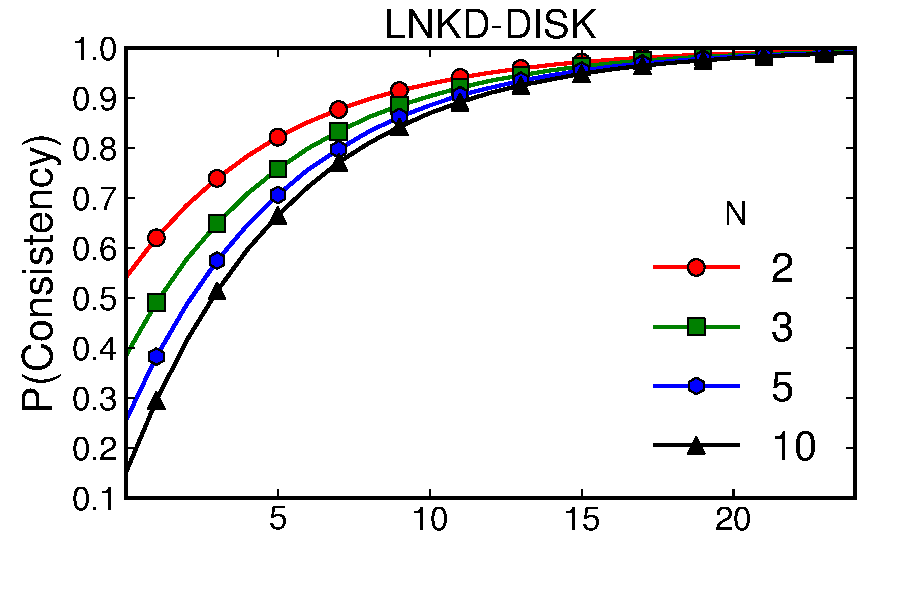
\includegraphics[width=.65\columnwidth]{figs/sweepn-lnkd-disk.pdf}}
\subfigure{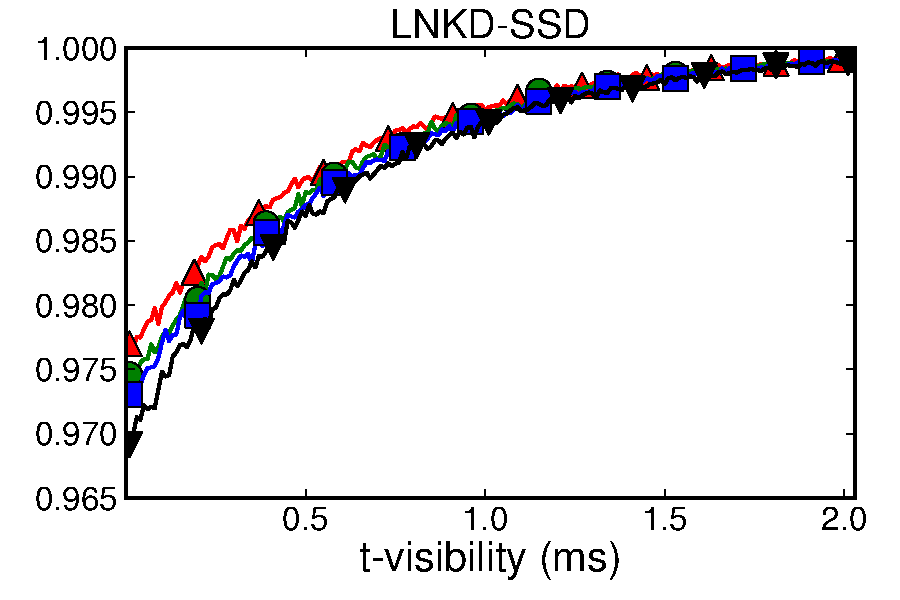
\includegraphics[width=.65\columnwidth]{figs/sweepn-LNKD-SSD.pdf}}
\subfigure{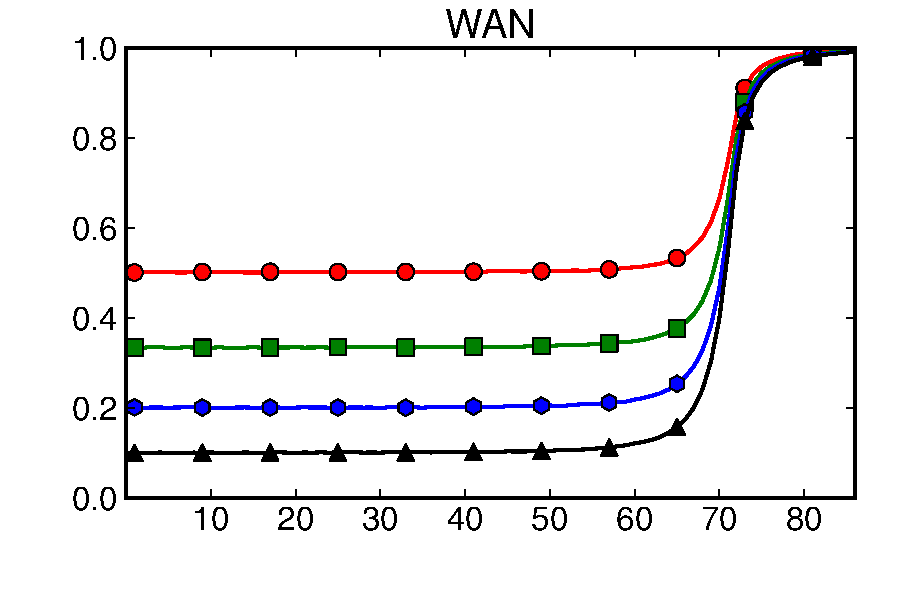
\includegraphics[width=.65\columnwidth]{figs/sweepn-WAN.pdf}}
\caption{$t$-visibility for production operating latencies for variable $N$ and $R$$=$$W$$=$$1$.}
\label{fig:varyn}
\end{figure*}

\subsection{Latency vs. $t$-visibility}

As we have discussed, choosing a value for $R$ and $W$ results in a
trade-off between operation latency and the $t$-visibility observed by
reads. To measure the obtainable latency gains, we studied
$t$-visibility required for a $99.9\%$ probability of consistent
reads, capturing the long tail of $t$-visibility.  We also measured
the $99.9$ percentile read, write latencies.
Table~\ref{table:lat-stale} shows the results for our latency
distributions and $R$, $W$ configurations.  For \texttt{YMMR}, we find
that though the best setting in terms of latency is $W$$=$$R$$=$$1$,
this configuration results in a high value for $t$-visibility: $1364$
ms. However, by setting $R$$=$$2$ and $W$$=$$1$, the $t$-visibility
reduces to $202$ ms and the combined read and write latencies decrease
by $81.1\%$ when with a compared to an overlapping quorum with
$W$$=$$1$, $R$$=$$3$.  Similarly, in the case of \texttt{LNKD-DISK} we
see that by adjusting the value of $R$ and $W$, combined read and
write latencies can reduce by $16.5\%$ with $t$-visibility of $13.6$
ms.  The write tail of \texttt{LNKD-SSD} was such that we never
observed message reordering for $R$$=$$2$, $W$$=$$1$, allowing a 30\%
latency reduction for no observable staleness (even across
$10,000,000$ writes).  $R$$=$$W$$=$$1$, reduced latency by $59.5\%$
with a corresponding $t$-visibility of $1.85$ ms.  Under \texttt{WAN},
$R$ or $W$ greater than one results in waiting for non-local
operations to complete and therefore large propagation time.  This
unsurprisingly results in staleness only when $R$$=$$W$$=$$1$.  These
results indicate that there are significant latency gains when to
employing lower values of $R$, $W$ and that $t$-visibility is can be
low even when we require a high percentage ($99.9\%$) of reads to be
consistent.

\begin{table*}
\centering
\begin{tabular}{c|c|c|c|c|c|c|c|c|c|c|c|c|}
\cline{2-13}
& \multicolumn{3}{|c|}{\texttt{YMMR}} & \multicolumn{3}{|c|}{\texttt{WAN}} & \multicolumn{3}{|c|}{\texttt{LNKD-SSD}} & \multicolumn{3}{|c|}{\texttt{LNKD-DISK}}\\
&\multicolumn{1}{|c}{$L_r$}  & \multicolumn{1}{c}{$L_w$} & \multicolumn{1}{c|}{$t$} &  \multicolumn{1}{|c}{$L_r$} & \multicolumn{1}{c}{$L_w$} & \multicolumn{1}{c|}{$t$} &  \multicolumn{1}{|c}{$L_r$} & \multicolumn{1}{c}{$L_w$} & \multicolumn{1}{c|}{$t$} &  \multicolumn{1}{|c}{$L_r$} & \multicolumn{1}{c}{$L_w$} & \multicolumn{1}{c|}{$t$} \\\hline
\multicolumn{1}{|c|}{$R$$=$$1$, $W$$=$$1$}
& 5.58 & 10.83 & 1364.0 & 3.4 & 55.12 & 113.0 & 0.66 & 0.66 & 1.85 & 0.66 & 10.99 & 45.5 \\
\multicolumn{1}{|c|}{$R$$=$$1$, $W$$=$$2$}
& 5.61 & 427.12 & 1352.0 & 3.4 & 167.64 & 0 & 0.66 & 1.63 & 1.79 & 0.65 & 20.97 & 43.3 \\
\multicolumn{1}{|c|}{$R$$=$$2$, $W$$=$$1$}
& 32.6 & 10.73 & 202.0 & 151.3 & 56.36 & 30.2 & 1.63 & 0.65 & 0 & 1.63 & 10.9 & 13.6 \\
\multicolumn{1}{|c|}{$R$$=$$2$, $W$$=$$2$}
& 33.18 & 428.11 & 0 & 151.31 & 167.72 & 0 & 1.62 & 1.64 & 0 & 1.64 & 20.96 & 0 \\
\multicolumn{1}{|c|}{$R$$=$$3$, $W$$=$$1$}
& 219.27 & 10.79 & 0 & 153.86 & 55.19 & 0 & 4.14 & 0.65 & 0 & 4.12 & 10.89 & 0 \\
\multicolumn{1}{|c|}{$R$$=$$1$, $W$$=$$3$}
& 5.63 & 1870.86 & 0 & 3.44 & 241.55 & 0 & 0.65 & 4.09 & 0 & 0.65 & 112.65 & 0 \\
\hline
\end{tabular}
\caption{$t$-visibility for $p_{staler} = .001$ ($99.9\%$ probability
  of consistency for $50,000$ reads and writes) and $99.9\%$ read
  ($L_r$) and write latency ($L_w$) across $R$ and $W$, $N$$=$$3$
  ($1M$ reads and writes).}
\label{table:lat-stale}
\end{table*}


\section{Discussion and Future Work}
\label{sec:discussion}

PBS enables several modifications to partial quorum systems that we
have not yet addressed.  Here, we briefly discuss them along with
improvements to our models.

\textbf{Latency/Staleness SLAs.} Using PBS, we can automatically
configure the configuration of replication parameters.  We can
optimize for operation latency given constraints on staleness and
minimum durability.  Data store operators can subsequently provide
service level agreements to applications and provide quantitative
trade-offs to developers, allowing them to reason about staleness
versus end-user latency.  Operators can determine configurations
analytically (and potentially revise them given online feedback).  PBS
provides a quantitative lens for analyzing consistency guarantees that
were previously unknown.  While this optimization formulation is
likely convex, the state space for configurations is rather small
($O(N^2)$).  This optimization also allows disentanglement of
replication for reasons of durability from replication for reasons of
low latency and higher capacity.  Operators can specify a minimum set
of nodes for druability and availability but may want to increase $N$,
which decreases tail latency for a fixed $R$ and $W$.

\textbf{Variable configurations.} We have assumed the use of a single
replica configuration ($N$, $R$, and $W$) across all operations.
However, one could consider varying these operations over time and
across keys, and many KVSs such as Cassandra and Riak allow the use of
per-operation consistency tuning at runtime.  By specifying an
\textit{average} operation latency, one could periodically modify $R$ and $W$ to
more efficiently guarantee a desired bound on staleness.  Similarly,
under scenarios with unexpectedly heavy load, one might consider
increasing the number of replicas and scaling $R$ and $W$ accordingly,
requiring additional refinements to our model, essentially revisiting
prior work on fluid replication~\cite{fluidreplication}.

\textbf{Stronger guarantees.} In this paper, we have limited our
discussions to probabilistic bounded staleness.  One might consider
analyzing the possibility that a data store provide a stronger yet
still eventually consistent guarantee such as causal consistency.
Predicting the probability of attaining more complex consistency
semantics requires additional modeling of application access patterns.
For example, to attain causal session guarantees, we would need to
know which replicas are contacted and whether clients inform one
another about causal relationships out-of-band from the data store.
This is possible, but modeling the \textit{worst-case} semantics of
these operations is likely to result in unfavorably low bounds on
consistency properties.  We can see this in Aiyer et al.'s analysis of
Byzantine $k$-quorums~\cite{multi-k-quorum}.  In a worst-case
deployment, with an adversarial scheduler, the lower bound on
staleness is quite high; we conjecture that the bound would be even
higher if the authors performed an analysis of stronger consistency
models.

\textbf{Alternative architectures.} We have analyzed Dynamo-style
$t$-visibility in depth.  As we discussed, Dynamo is conceptually easy
to understand (\textit{WARS}) and implement but is painful to analyze
analytically, leading us to favor Monte Carlo analysis.  Dynamo is
surprisingly resilient to inconsistency in practice, but attaining
\textit{provable} (even probabilistically provable) $t$-staleness
bounds would be desirable for applications that cannot tolerate
statistical error.  While research on deterministic bounded staleness
(Section~\ref{sec:relatedwork}) provides provably deterministic bounds
(often sacrificing availability), it is unclear whether there is a
design that finds the middle ground between operational elegance and
easy, provable analysis in the eventually consistent protocol design
space.

\textbf{Multi-key operations.} We have considered single-key
operations, however the ability to perform multi-key operations is
potentially attractive.  For read-only transactions, if the key
distribution is random and each quorum is independent, we can simply
multiple the staleness probabilities of each key.  Achieving atomicity
of writes to multiple keys requires more complicated coordination
mechanisms such as two-phase commit, increasing operation latency.
Transactions are feasible but require considerable care in
implementation, complicating what is otherwise a simple replication
scheme.

\textbf{Failure modes.} In our evaluation of $t$-visibility, we
focused on normal operating conditions. Unless failures are
common-case, they affect $p_{stale}$ at the tail.  If, as Jeff Dean of
Google suggests~\cite{dean-keynote}, servers crash at least twice per
year, assuming a worst-case ten hour downtime for machines, this
roughly represents .23\% downtime per machine.  If failures are
correlated, this small percentage may be a problem.  If they are
independent, a replica set of $N$ failed nodes with $F$ failed nodes
behaves like an $N-F$ replica set, and the probability of all $N$
nodes failing is $(.23)^N$\% (``five nines'' reliability for
$N$$=$$3$).  However, it would be beneficial to quantify this impact
more precisely given actual failure distributions.  We have asserted
that failures or latency spikes can be accommodated in \textit{WARS}
by adjusting latency distributions to match failure probabilities.
However, modeling the probability of treating replicas as inactive
(while it is just hung) and modeling recovery semantics such as hinted
handoff would be fruitful.  This requires additional information about
failure rates and additional care in gathering latency distributions.

\section{Related Work}
\label{sec:relatedwork}

We surveyed quorum replication
techniques~\cite{prob-quorum-dynamic,non-strict, multi-k-quorum,
  quorum-start,quorum-placement, quorums-alternative, prob-quorum,
  quorum-overview, quorumsystems} in Section~\ref{sec:background}.  In
this work, we specifically draw inspiration from probabilistic
quorums~\cite{prob-quorum} and deterministic
$k$-quorums~\cite{multi-k-quorum, non-strict} in analyzing
write-propagating quorum systems and their staleness.  We believe that
revisiting probabilistic quorum systems---including non-majority
quorum systems such as tree quorums---in the context of write
propagation, dynamism, and Dynamo is a promising area for theoretical
work.

Data consistency is a long-studied problem in distributed
systems~\cite{consistency-partitioned, danger-rep} and concurrent
programming~\cite{linearizability}.  Given the CAP Theorem and the
inability to maintain all three of consistency, availability, and
partition tolerance~\cite{cap-proof}, data systems have turned to
``eventually consistent'' semantics to provide availability in the
face of partitions~\cite{consistency-partitioning, vogels-defs}.
Real-time consistency (RTC) is the strongest consistency model
available in an available, one-way convergent (eventually consistent)
system~\cite{rtc-proof}, however there is a plethora of alternative
consistency models offering various performance tradeoffs, from
session guarantees~\cite{sessionguarantees} to causal+
consistency~\cite{cops} and parallel snapshot isolation~\cite{walter}.
Instead of proposing a new consistency model and building a system
implementing new semantics, we have examined what consistency
existing, widely deployed quorum-replicated systems actually provide.

There are several systems that provide deterministic bounds on
staleness.  FRACS~\cite{frac} allows replicas to buffer updates up to
a given staleness threshold under several replication schemes,
including master-drive and group gossip.  AQuA~\cite{aqua}
asynchronously propagates updates from a designated master to replicas
that in turn serve reads depending on probabilistic models regarding
their staleness.  AQuA actively selects which replica to contact
depending on the staleness bound and replica staleness predictions.
TRAPP~\cite{trapp} provides tradeoffs between precision and
performance for continuously evolving numerical data.  In
TACT~\cite{vahdat-article, vahdat-bounded} consistency is modeled
according to numerical error, order error, and staleness.  TACT bounds
staleness by ensuring that each replica makes (transitive) contact
with all other replicas in the system within a given time window.
Finally, PIQL~\cite{piql} bounds the number of operations performed
per query, trading operation latency at scale with the amount of data
a particular query can access, potentially impacting accuracy.

In this work, we analyze quorum replication systems and study the
properties real-world Dynamo-style quorum systems in depth.  Many of
the aforementioned deterministic bounded staleness systems represent the
deterministic dual of PBS, and their bounding algorithms could likely
be employed in a write-all quorum system like Dynamo.

\section{Conclusion}
\label{sec:conclusion}

In this paper, we developed models for the staleness of values
returned from eventually consistent quorum-replicated data stores.  By
extending prior theory on probabilistic quorum systems, we derived an
analytical solution for the $k$-staleness of a partial quorum system,
representing the expected staleness of a read operation in terms of
versions.  We analyzed the $t$-visibility, or expected staleness of a
read in terms of real time, under Dynamo-style quorum replication.  To
do so, we developed the the \textit{WARS} latency model to explain how
message reordering leads to staleness under Dynamo.  To examine the
effect of latency on $t$-staleness in practice, we used real-world
traces from internet companies to drive a Monte Carlo analysis.  We
find that eventually consistent quorum-replicated data stores are
frequently consistent after only a few milliseconds, explaining the
prevalence of partial-quorum operation configurations in practice.  We
conclude that ``eventually consistent'' partial quorum replication
schemes frequently deliver consistent semantics in practice due largely to the
resilience of Dynamo-style messaging.

\section*{Interactive Demonstration}

An interactive demonstration of Dynamo-style PBS is available online at \url{http://cs.berkeley.edu/~pbailis/pbs/}.  The username is \texttt{demo} and the password is \texttt{vldborbust}.

\section*{Acknowledgements}

The authors would like to thank Alex Feinberg and Coda Hale for their
cooperation in providing real-world distributions for experiments and
exemplifying positive industrial-academic relations in their actions
and assistance.

The authors would also like to thank the following individuals whose
discussions and feedback improved this work: Marcos Aguilera, Peter
Alvaro, Eric Brewer, Neil Conway, Greg Durrett, Hariyadi Gunawi, Bryan
Kate, Sam Madden, Bill Marczak, Kay Ousterhout, Christopher R\'e,
Scott Shenker, Sriram Srinivasan, Doug Terry, Greg Valiant, and
Patrick Wendell, \textbf{YOUR NAME HERE, BOLD READER}!  We would
especially like to thank Ali Ghodsi, who, in addition to providing
feedback, originally piqued our interest in theoretical quorum
systems.

This work was supported in part by AMPLab gifts from Google, SAP,
Amazon Web Services, Cloudera, Ericsson, Huawei, IBM, Intel,
MarkLogic, Microsoft, NEC Labs, NetApp, Oracle, Splunk, and VMware and
by DARPA (contract \#FA8650-11-C-7136).  This material is based upon
work supported by the National Science Foundation Graduate Research
Fellowship under Grant No. DGE 1106400.


\begin{comment}
Andy Gross
Justin Sheehy


\end{comment}

\balance

\footnotesize
\bibliographystyle{abbrv}
\bibliography{ernst}

\begin{appendix}
\section{PBS Quorum Load}
The theoretical quorum literature describes the \textit{load} of a quorum
system as a metric for the frequency of accessing the busiest quorum
member~\cite[Definition 3.2]{quorumsystems}.  Intuitively, the busiest
quorum member limits the number of requests, or capacity, that a given
quorum system can sustain~\cite[Corollary 3.9]{quorumsystems}.

Prior work determined that probabilistic quorum systems did not offer
significant benefits to load (a constant factor improvement compared
to strict quorum systems)~\cite{prob-quorum}.  Here, we show that PBS
$k$-quorums provide asymptotically lower load than traditional
probabilistic quorum systems (and, transitively, than strict quorum
systems).

The probabilistic quorum literature defines an
$\varepsilon$-intersecting quorum system as a quorum system that
provides a $1-\varepsilon$ probability of returning consistent
data~\cite[Definition 3.1]{prob-quorum}.  A $\varepsilon$-intersecting
quorum system has a lower bound load of
$\frac{1-\sqrt{\varepsilon}}{\sqrt{N}}$~\cite[Corollary
  3.12]{prob-quorum}.

By considering $k$ versions of staleness, we are considering the
intersection of multiple $\varepsilon$-intersecting quorum systems.
However, for a given probability $p$ of inconsistency, if we are
willing to tolerate $k$ versions of staleness, we need only require
that that $\varepsilon = \sqrt[k]{p}$.  This implies that our PBS
$k$-quorum system construction has load no less than
$\frac{(1-p)^{\frac{1}{2k}}}{\sqrt{N}}$, a lower bound than
traditional probabilistic quorum systems.  PBS monotonic reads results
in a lower bound on load of $\frac{(1-p)^{\frac{1}{2C}}}{\sqrt{N}}$, where
$C=1+\frac{\gamma_{gw}}{\gamma_{cr}}$.

These results are intuitive: if we are willing to tolerate multiple
versions of staleness, we need to contact fewer replicas.  However, we
believe this is the first formal demonstration that staleness
tolerance lowers load on quorum members, raising quorum system
capacity.


\end{appendix}


\end{document}

